\section{Observer}
\subsection{Descrizione}
Il pattern Observer, noto anche col nome \textit{Publish-Subscriber}, permette di definire una dipendenza uno a molti fra oggetti, in modo tale che se un oggetto cambia il suo stato interno, ciascuno degli oggetti dipendenti ad esso viene notificato e aggiornato automaticamente.

\subsection{Struttura}
\begin{figure}[H]
\centering
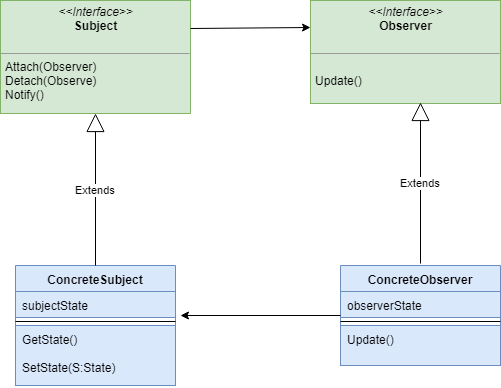
\includegraphics[scale=0.6]{images/observer}
\caption{Struttura observer\label{fig:UC3}}
\end{figure}
\begin{itemize}
	\item \textbf{Subject}
	\begin{itemize}
		\item Il Subject è l'oggetto che notifica li observers;
		\item Il Subject conosce i suoi Observer perchè possiede un riferimento ad essi;
		\item Il metodo \textit{Attach()} serve a sottoscrivere un nuovo observer;
		\item Il metodo \textit{Detach()} serve ad eliminare un observer;
		\item Il metodo \textit{Notify()} sarà implementato dagli observers.
	\end{itemize}
	\item \textbf{ConcreteSubject}
	\begin{itemize}
		\item Quando ConcreteSubject cambia Stato, avverte tutti i ConcreteObserver, attraverso l'invocazione del metodo \textit{Notify()}, ereditato da Subject;
	\end{itemize}
		\item \textbf{Observer}
	\begin{itemize}
		\item Il metodo \textit{Update()} dev'essere implementato dai ConcreteObservers;
	\end{itemize}
	\item \textbf{ConcreteObserver}
	\begin{itemize}
		\item Implementa il metodo \textit{Update()} di Observer;
	\end{itemize}
\end{itemize}

\subsection{Esempio 1}

 Modifica di una o più aree di finestre in risposta alla pressione di un pulsante
\begin{figure}[H]
\centering
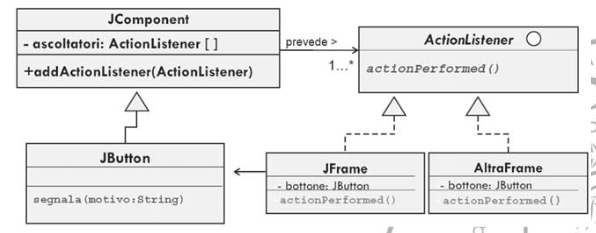
\includegraphics[scale=0.8]{images/esempio1Observer}
\caption{Struttura observer\label{fig:UC3}}
\end{figure}
\begin{itemize}
	\item \textbf{JComponent} agisce da Subject;
	\item \textbf{ActionListener} agisce da Observer;
	\item \textbf{JButton} rappresenta il concreteObserver. È colui che fa scaturire la notifica;
	\item \textbf{JFrame e Altra Frame} rappresentano i concreteObserver;
	\item i 2 concreteObserver hanno un riferimento al concreteSubject ed implementano il metodo \textit{actionPerformed} ereditato da ActionListener;
	\end{itemize}